\documentclass{article}%You can define the type of paper here.
%%Useful packages that I commonly use.
\usepackage{cite}%Bibliography package (help at http://merkel.zoneo.net/Latex/natbib.php).
\usepackage{url}%Package to highlight url.
\usepackage{times}%Sets font to be times.
\usepackage{siunitx}
\usepackage{alltt}%Allows the use of verbatim (good for printing out code).
\usepackage{graphicx}%Used to import images.
\usepackage{amsmath, amssymb, amscd}%Contains the AMS expanded math symbols library.
\usepackage{algorithm, algorithmic} %pseudo-code
%%For those who want smaller margins, you can use this:
\usepackage[top=1in, bottom=1in, left=1in, right=1in]{geometry}
\newcommand{\sups}[1]{\ensuremath{^{\textrm{#1}}}}
\newcommand{\subs}[1]{\ensuremath{_{\textrm{#1}}}}

\makeatletter
\renewcommand\@biblabel[1]{\textbullet}
\makeatother

\begin{document}

%% Title =======================================================================

\title{Firn densification model}
\author{Douglas Brinkerhoff \and Evan Cummings \and Tyler Davis \and Jesse Johnson}
\maketitle
\begin{center}

\includegraphics[width=4.455666122085252in]{images/logoPlain.png}
\end{center}

\twocolumn


%% Introduction ================================================================
\section{Introduction}

The top layer of snow on a glacier or ice sheet increases in density as depth increases; newly accumulated snow builds up and compresses the layers below.  \emph{Herron and Langway} [1980] developed a firn densification model based on Arrhenius-type equations with variable rate constants, and found that the densification rate decreased suddenly around $550$ kg m\sups{-3}.  \emph{Zwally and Li} [2002] expanded upon this model and found an alternate temperature-dependent value for the rate constant.  \emph{Arthern et al.} [2010] developed yet another set of equations based from their in situ measurements of Antarctic snow compaction.  \emph{Ligtenberg et al.} [2011] modified the \emph{Arthern et al.} [2010] parametrization to better fit areas with a higher average annual temperature. 

We have re-created a number of these models and integrated them with an enthalpy-formulation proposed by \emph{Aschwanden et al.} [2012] which accounts for melting of firn layers in percolation zones.  The model simulates ice lenses formed from within the firn column, and work is currently being done to allow the movement of water through the column.  The model has been created with the finite-element software package FEniCS; an explanation of its usage and flexibility will be made clear.

%% Temperature =================================================================
\section{Temperature Solution}

We begin with the standard heat-transport equation as explained by \emph{Patterson} [2001]

  $$
  \rho c_i \frac{\partial T}{\partial t} = 
    k_i \frac{\partial^2 T}{\partial z^2} +
    \left( \frac{dk_i}{dt} - \rho c_i w \right) \frac{\partial T}{\partial z}
  $$
with heat sources from the deformation of ice omitted, $\rho$ density, $c_i$ heat capacity, $k_i$ thermal conductivity, $w$ vertical velocity, and $T$ temperature of firn.  To solve the total derivative $dk_i/dt$ we must apply the chain rule
  $$
  \frac{dk_i}{dz} = 
  \frac{\partial k_i}{\partial \rho} \frac{\partial \rho}{\partial z} + 
  \frac{\partial k_i}{\partial T} \frac{\partial T}{\partial z}.
  $$
The thermal conductivity of ice is defined by \emph{Arthern et. al, 1998} as
  $$k_i = 2.1 \left(\frac{\rho}{\rho_i}\right)^2,$$
from which we find
  $$
  \frac{\partial k_i}{\partial \rho} = 
    4.2 \frac{\rho}{\rho_i^2}
  $$
and
  $$
  \frac{\partial k_i}{\partial T} = 
    \frac{4.2}{\rho_i^2} \left( \frac{\partial \rho}{\partial T} \right).
  $$
\emph{Patterson} [2001] defined the heat capacity $c_i$ of firn with the equation
  $$
  c_i = 152.5 + 7.122 T,
  $$
and also defined $\rho$ in terms of $T$ which leads to the equation:
  $$
  \frac{\partial \rho}{\partial T} = 
    (\SI{5.6e-2}) \exp ((\SI{-5.7e-3})T).
  $$
The vertical velocity of ice $w$ can be described with the differential equation
  $$
  \frac{\partial w}{\partial z} = \frac{1}{\rho} \frac{d \rho}{dt}.
  $$


%% Density =====================================================================
\section{Density Solution}

The densification process is defined with the material derivative
  $$\frac{d \rho}{dt} = \frac{\partial \rho}{\partial t} + 
    w\frac{\partial \rho}{\partial z}.$$
\emph{Arthern et al.} [2010] described this derivative differently for density values above and below a critical value, $\rho_m$:  
  $$
  \frac{d \rho}{dt} = 
  \begin{cases}
   c_0(\rho_i - \rho), &\rho \leq \rho_m\\
   c_1(\rho_i - \rho), &\rho > \rho_m
  \end{cases}.$$
\emph{Zwally and Li} [2002] defined a single multiplying constant $c$ with an Arrhenius-type relation
  $$
  c_0 = c_1 = 
  \dot{b} \beta(T)\left(\frac{\rho_i}{\rho_w}\right)
  K_{0G}(T)\exp \left( -\frac{E(T)}{RT} \right),
  $$
with $K_{0G}(T) \exp(-E(T)/(RT)) = 8.36T^{-2.061}$ as described in \emph{Reeh} [2008], accumulation rate $\dot{b}$ in units of kg m\sups{-2} s\sups{-1}, and $\beta(T)$ a unit-less smoothing function to match a desired density rate.  \emph{Arthern et al} [2010] developed a semi-empirical formula by coupling the rate equations for Nabarro-Herring creep and normal grain-growth: 
  $$
  \begin{cases}
    c_0 = M_0 \dot{b}g\frac{k_{c0}}{k_g}\exp\left(-\frac{E_c}{RT} + 
          \frac{E_g}{RT_{avg}}\right)\\
    c_1 = M_1 \dot{b}g\frac{k_{c1}}{k_g}\exp\left(-\frac{E_c}{RT} + 
          \frac{E_g}{RT_{avg}}\right)
  \end{cases},
  $$
with the creep coefficients defined as
  $$
  \begin{cases}
    k_{c0} = \text{\SI{9.2e-9} m\sups{3} s kg\sups{-1}} \\
    k_{c1} = \text{\SI{3.7e-9} m\sups{3} s kg\sups{-1}}  
  \end{cases}
  $$
and $M$ defined in \emph{Ligtenberg et al.} [2011] to better fit with observed densification rates in higher-temperature environments:
  $$
  \begin{cases}
    M_0 = 2.366 - 0.293\ln(\dot{b}*\SI{1e3})\\
    M_1 = 1.435 - 0.151\ln(\dot{b}*\SI{1e3})
  \end{cases}.
  $$
Within the same paper a firn surface-density expression from data was given:
  $$ \rho_s = -151.94 + 1.4266(73.6 + 1.06T_s + 0.0669A + 4.77V_a).$$


%% Enthalpy ====================================================================
\section{Enthalpy Solution}

As stated in \emph{Aschwanden et al.} [2012], we take 'enthalpy' to be synonymous with 'internal energy' due to the exclusion of work done with changing volume.  The equation used here is the shallow-enthalpy:
	$$
  \rho \frac{\partial H}{\partial t} = \frac{\partial}{\partial z} 
    \left( 
      \begin{Bmatrix}
        K_i, &\text{Temperate}\\
        K_0, &\text{Cold}
      \end{Bmatrix}
      \frac{\partial H}{\partial z} 
    \right) + w \rho \frac{\partial H}{\partial z}.
  $$
Strain heating has been neglected and the advective term $w \rho\ \partial H / \partial z$ has been added.  The coefficient for temperate ice is 
  $$K_i = \frac{k_i}{c_i},$$
and the coefficient for cold ice is
  $$K_0 = \frac{1}{10}K_i.$$
Temperate firn is defined as firn with $H > H_s$, cold firn with $H \leq H_s$, where
  $$H_s = \int_{T_0}^{T_m}{c_i(T)}dT,$$ 
with $T_m = 273.15$ K and $T_0 = 0.0$ K.  The enthalpy can be found with a constant heat capacity of $2009$ J kg\sups{-1} K\sups{-1} by the linear equation
  $$
  H = 
  \begin{cases}
    c_i(T - T_0), &\text{where } T \leq T_m\\
    c_i(T_w - T_0) + \omega L_f,  &\text{where } T > T_m
  \end{cases}
  $$
where $L_f$ is the latent heat of fusion and $\omega$ represents the water content percentage of firn given by
  $$\omega L_f = H - c_i(T_w - T_0).$$
Temperature may be derived from enthalpy easily:
  $$T = \frac{H}{c_i}.$$
The density of the firn column changes with the percentage of water content:
  $$
  \rho^n = 
  \begin{cases}
    \rho^{n-1} + \Delta\omega(\rho_w - \rho_i)\ \text{kg m\sups{-3}},  
      &\Delta\omega \leq 0\\
    \rho^{n-1} + \Delta\omega\rho_w\ \text{kg m\sups{-3}}, 
      &\Delta\omega > 0
  \end{cases},
  $$
where $\Delta\omega = \omega^n - \omega^{n-1}$ is the change in water content and superscripts refer to the time index.  This has the effect of adding water to the firn column and refreezing the portion of firn with decreasing water content.  The surface-density at time index $n+1$ can be described as: 
  $$\rho_s^{n+1} = \rho_{\dot{b}}^{n+1} d_p + \rho_s^{n} (1 - d_p),$$
where
  $$\rho_{\dot{b}}^{n+1} = \rho_{\dot{b}}^{n-1} + \Delta \omega_s \rho_{\dot{b}}^n,$$
  $$\Delta \omega_s = \omega_s^{n} - \omega_s^{n-1},$$ 
  $$d_p = \frac{d_n}{l_s},$$
  $$d_n = w_s\Delta t,\text{ and}$$
  \begin{center}$l_s$ is the length of the surface node.\end{center}
If $T_s \geq T_w$, the density of surface snow while taking into account re-freezing is simulated making
  $$
  \rho_{\dot{b}}^n = 
  \begin{cases}
    \rho_w - \rho_i\ \text{kg m\sups{-3}},  &\Delta\omega_s < 0\\
    \rho_w\ \text{kg m\sups{-3}}, &\Delta\omega_s > 0\\
  \end{cases},
  $$
but when $T_s < T_w$, $\rho_{\dot{b}}^n$ is simply made to be $\rho_{si}$.
\begin{figure}[H]
	\centering
		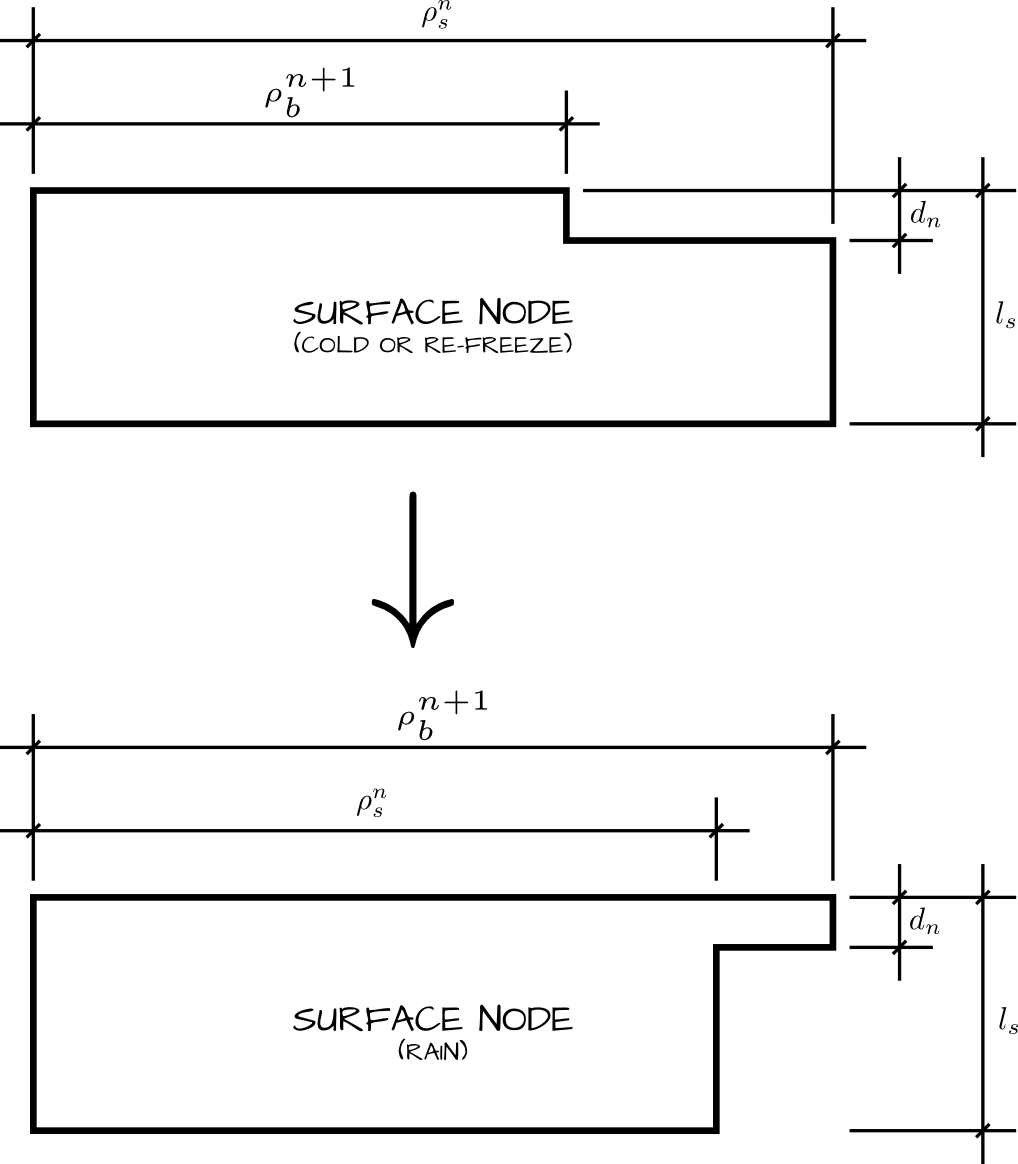
\includegraphics[width=0.42\textwidth]{images/surfaceDensity.png}
	\label{fig:500 year orbit}
	\caption{Evolution of surface node density}
\end{figure}


%% Age =========================================================================
\section{Age Solution}

The age of firn is described with the equation
  $$
  \frac{\partial a}{\partial t} = 1 - w \nabla{a}.
  $$
Because this equation is purely advective, upwinding is needed.  The Taylor series expansion of $w$ is
  $$
  a^{k+1} = a^{k} + \frac{\partial a^k}{\partial t}\Delta t + 
            \frac{1}{2}\frac{\partial^2 a^{k+\theta}}{\partial t^2}\Delta t^2 + 
            \mathrm{O} (\Delta t^3).
  $$
Replacing the time partials with the previous equation and eliminating the $\Delta t^3$ term, we have
  $$
  a^{k+1} = a^{k} + \left[1 - w \nabla{a}^k \right] \Delta t
            - \frac{1}{2}\frac{\partial}{\partial t}
              \left[1 - w \nabla{a}^{k+\theta} \right] \Delta t^2. 
  $$
Rearranging and simplifying,
  $$
  \frac{a^{k+1} - a^{k}}{\Delta t} = 1 - w \nabla{a}^k
        - \frac{w \Delta t}{2} 
          \left( \nabla \frac{\partial a^{k+\theta}}{\partial t} \right).
  $$
The time differential in the last term can again be replaced, 
  $$
  \frac{a^{k+1} - a^{k}}{\Delta t} = 1 - w \nabla{a}^k
        - \frac{w \Delta t}{2} 
          \left( \nabla [1 - w \nabla a^{k+\theta}] \right),
  $$
and reduced to
  $$
  \frac{a^{k+1} - a^{k}}{\Delta t} = 1 - w \nabla{a}^k
        + \frac{w \Delta t}{2} 
          \left( \nabla w \nabla^2 a^{k+\theta} \right).
  $$
With $\theta=0$ and factoring,
  $$
  \frac{a^{k+1} - a^{k}}{\Delta t} = 1 + w \nabla{a}^k 
     \left(\frac{\Delta t}{2} \nabla w \nabla a^{k} - 1 \right).
  $$
Multiplying by the test function $\xi$ and integrating over $\Omega$ we have
  $$
  0 = \int_{\Omega} \frac{a^{k+1} - a^{k}}{\Delta t}\xi\ d\Omega - 
      \int_{\Omega} 1\xi\ d\Omega +
  $$
  $$ 
      \int_{\Omega} w \nabla{a}^k \xi\ d\Omega
      - \int_{\Omega} \frac{w \Delta t}{2} 
      \left( \nabla w \nabla^2 a^{k+\theta} \right)\xi\ d\Omega.
  $$
Integrating the last term by parts and disregarding the boundary term results in
  $$
  0 = \int_{\Omega} \frac{a^{k+1} - a^{k}}{\Delta t}\xi\ d\Omega - 
      \int_{\Omega} 1\xi\ d\Omega
  $$
  $$ 
  + \int_{\Omega} w \nabla{a}^k \xi\ d\Omega
      + \int_{\Omega} \frac{w \Delta t}{2} 
      \left( \nabla w \nabla a^{k+\theta} \right)\nabla \xi\ d\Omega.
  $$


%% Method ======================================================================
\section{Finite Element Method}

This section will focus on the enthalpy solution.  Solving these equations with FEniCS is done with Galerkin's method and requires finding the weak formulation:
  $$
    0 =
    \int_{\Omega} 
      \begin{Bmatrix}
        K_i\\
        K_0
      \end{Bmatrix}
      \nabla^2 H \psi\ d \Omega 
    + \int_{\Omega}w \rho \nabla H \psi\ d \Omega
  $$
  $$
    - \int_{\Omega} {\rho \frac{\partial H}{\partial t}} \psi\ d \Omega.
  $$
Here we have integrated the enthalpy equation over the entire domain, $\Omega$, and multiplied by a test function $\psi$.  After integrating the diffusive term by parts this becomes
  $$
    f_H =
    - \int_{\Omega} 
        \begin{Bmatrix}
          K_i\\
          K_0
        \end{Bmatrix}
        \nabla H \nabla \psi\ d \Omega 
    + \int_{\Omega}w \rho \nabla H \psi\ d \Omega
  $$
  $$
    - \int_{\Omega} {\rho \frac{\partial H}{\partial t}} \psi\ d \Omega.
  $$
We can discretize the enthalpy time-differential with the second-order accurate formula
  $$\frac{\partial H}{\partial t} = \frac{H - H^{k-1}}{\Delta t} = \theta H^{k}  + (1-\theta) H^{k-1}$$
with superscripts referring to time index.  Using a $\theta$-scheme as given by \emph{Logg et al.} [2011], $H_{mid} = \theta H^{k}  + (1-\theta) H^{k-1}$, where $\theta \in [0,1]$ is a weighting factor chosen from: 
  $$
    \theta = 
    \begin{cases}
      1,       & \text{Backwards-Euler}\\
      0.667,   & \text{Galerkin}\\
      0.878,   & \text{Liniger}\\
      0.5,     & \text{Crank-Nicolson}\\
      0,       & \text{Forward-Euler}\\
    \end{cases}
  $$
The entire enthalpy residual can be represented in FEniCS as:\par
\footnotesize
\begin{alltt}
theta = 0.5
H_mid = theta*H + (1 - theta)*H_1
f_H   = rho*(H - H_1)/dt*psi*dx + 
        k/c*Kcoef*
        inner(grad(H_mid), grad(psi))*dx + 
        rho*w*grad(H_mid)*psi*dx
\end{alltt}
\normalsize
The variable \texttt{Kcoef} is a coefficient vector which will be updated dynamically depending on the temperature of firn (either $1.0$ or $0.1$ corresponding to $K_i$ and $K_0$).

The weak form for density is found similarly, with a upwinding necessary to eliminate artifacts due to the sudden increase in density where ice lenses formed.  The method used here is the Streamline Upwind Petrov-Galerkin (SUPG) method:
  $$
    \hat{\phi} = \phi + \frac{h}{2||w||} w \cdot \nabla{\phi},
  $$
where $h$ is the cellsize.  The density residual after integration by parts becomes:
  $$
  f_{\rho} = 
    \int_{\Omega} \frac{\partial \rho}{\partial t}\phi\ d \Omega + 
    \int_{\Omega} w\nabla \rho \hat{\phi}\ d \Omega -
    \int_{\Omega}\frac{d \rho}{dt}\hat{\phi}\ d \Omega.
  $$
With the partial-time differential of density defined identically to the enthalpy equation, this can be represented in FEniCS including the \emph{Arthern et al.} [2010] densification equation as:\par
\footnotesize
\begin{alltt}
vnorm   = sqrt(dot(w, w) + 1e-10)
cellh   = CellSize(mesh)
phihat  = phi + cellh/(2*vnorm)*dot(w, grad(phi))
c       = b*g*rhoCoef/kg * 
          exp(-Ec/(R*T) + Eg/(R*Tavg))
drhodt  = c*(rhoi - rho)
theta   = 1.0
rho_mid = theta*rho + (1 - theta)*rho_1
f_rho   = (rho - rho_1)/dt*phi*dx - 
          (drhodt - w*grad(rho_mid))*phihat*dx
\end{alltt}
\normalsize
The variable \texttt{rhoCoef} is another dynamically-updated-coefficient vector and is either $k_{c0}$ or $k_{c1}$ depending upon the density at the node.  We have chosen $\theta = 1$ corresponding to the Backwards-Euler method due to the jump condition at $\rho_m$.

In order to find the vertical velocity the differential equation must be solved.  The weak formulation is:
  $$
  f_{w} = 
    \int_{\Omega} \rho \nabla{w} \eta\ d\Omega + \frac{d\rho}{dt} \eta\ d\Omega,
  $$
and is created with FEniCS by:
\footnotesize
\begin{alltt}
theta     = 1.0
w_mid     = theta*w + (1 - theta)*w_1
f_w       = rho*grad(w_mid)*eta*dx + drhodt*eta*dx
\end{alltt}
\normalsize
We chose $\theta=1$ again due to the jump discontinuity at $\rho_m$.


We can define the function space for the entire non-linear problem as 
  $$
    U = \Omega \times \Omega \times \Omega,
  $$
with corresponding trial and test functions respectively defined as
  $$
    d_h, j \subset U.
  $$
The test functions for each function can now be described as
  $$
    \psi, \phi, \eta \subset j.
  $$
In FEniCS these spaces can be defined by this:
\footnotesize
\begin{alltt}
mesh        = IntervalMesh(n, zb, zs)
V           = FunctionSpace(mesh, 'Lagrange', 1)
MV          = MixedFunctionSpace([V, V, V])
h           = Function(MV)
H,rho,w     = split(h)    
dh          = TrialFunction(MV)
dH,drho,dw  = split(dh)
j           = TestFunction(MV)
psi,phi,eta = split(j)
\end{alltt}
\normalsize
The variable \texttt{zb} is the z-position of the base of the firn column which does not change and \texttt{n} is the number of nodes; the \texttt{mesh} variable defines the spacial dimensions of the system to be solved and is here created in one dimension.  The mesh may also be created in three dimensions if desired, or made to fit a custom grid.  The variables \texttt{dH} and \texttt{drho} are the trial functions for the enthalpy and density functions and are not utilized in this code, but are included for reference later on.

We define the complete non-linear residual as 
  $$
    f = f_H + f_{\rho} + f_w.
  $$
Solving this system can be accomplished with \emph{Newton's Method} which requires derivation of the Jacobian:
  $$
    J = \frac{\partial f}{\partial d_h}.
  $$
In FEniCS this is done with:
\footnotesize
\begin{alltt}
f  = f_H + f_rho + f_w
J  = derivative(f, h, dh)
\end{alltt}
\normalsize


%% Boundary Conditions =========================================================
\section{Boundary Conditions}

A cyclical enthalpy boundary condition for the surface can be simulated with 
  $$
    H_s = c_i ( T_s - T_0 ),
  $$
  $$
    T_s = T_{avg} + \alpha \sin(\omega t),
  $$
where $\alpha$ is the amplitude of temperature variation and $\omega = 2\pi / spy$ is the frequency.  The surface-density boundary condition can be likewise described as (see Figure 1): 
  $$
    \rho_s^{n+1} = \rho_{\dot{b}}^{n+1} d_p + \rho_s^{n} (1 - d_p).
  $$
Both of these can be created with FEniCS by
\footnotesize
\begin{alltt}
code = 'c*(Tavg + 9.9*sin(omega*t) - T0)'
Hs   = Expression(code, c=cp, Tavg=Tavg, 
                  omega=freq, t=t0, T0=T0)

code = 'dp*rhon + (1 - dp)*rhoi'
rhoS = Expression(code, rhon=rhosi, 
                  rhoi=rhosi, dp=1.0)

def surface(x, on_boundary):
  return on_boundary and x[0] == zs

Hbc  = DirichletBC(MV.sub(0), Hs, surface)
Dbc  = DirichletBC(MV.sub(1), rhoS, surface)
\end{alltt}
\normalsize
Within the time-loop the variables \texttt{t}, \texttt{rhon}, \texttt{rhoi}, and \texttt{dp} can be updated as needed.

Now all that is left is to iterate through time and call the \texttt{solve} method at each step:\par
\footnotesize
\begin{alltt}
solve(f == 0, h, [Hbc, Dbc], J=J)
\end{alltt}
\normalsize
The use of the \texttt{solve} function in this way chooses \emph{Newton's Method} by default and minimizes the residual of \texttt{f}.  The boundary conditions are updated by specifying the list \texttt{[Hbc, Dbc]}.


%% Model Parameters ============================================================
\section{Model Parameters}

Within the time-loop there are a number of parameters which need to be updated.  Taking into account conservation of mass, the height $l$ of each node must be re-calculated:\par
  $$l_{new} = l_{ini} \frac{\rho_{ini}}{\rho},$$
where $\rho_{ini}$ abd $l_{ini}$ are the density and height vectors of the firn column when the system was initialized.  With the height of the nodes calculated, the z-positions may be found by iterating through the heights and setting the z vector's corresponding cell equal to the current sum.  After successful calculation the FEniCS \texttt{mesh} object must have its coordinates refreshed.  These tasks may be completed with the following code:\par
\footnotesize
\begin{alltt}
lnew     = l*rhoin / firn.rho
zSum     = zb
zTemp    = zeros(n)
for i in range(n)[1:]:
  zTemp[i] = zSum + lnew[i]
  zSum    += lnew[i]
firn.z  = zTemp
mesh.coordinates()[:,0][index] = firn.z
\end{alltt}
\normalsize
The variable \texttt{index} is an array of positions corresponding to the correct ordering of the nodes, necessary after mesh refinement.  

The height $s$ at time index $n$ of the original surface may be calculated as follows:
  $$s^{n} = (z_s^0 - z_b) \frac{s^{n-1} - z_b}{z_s^{n-1} - z_b} + w_s \Delta t.$$
This maintains the relative location of the original surface to the current surface and moves downward proportional to $w$.  This is accomplished in Python with\par
\footnotesize
\begin{alltt}
interp     = interp1d(firn.z, 
                      firn.w,
                      bounds_error=False,
                      fill_value=firn.w[0])
zint       = array([firn.origZ])
wOrigZ     = interp(zint)
firn.origZ = (firn.z[-1] - zb) * 
             (firn.origZ - zb) / 
             (zs_0 - zb) + wOrigZ[0] * dt
\end{alltt}
\normalsize
The second index for \texttt{firn.z} refers to the surface, \texttt{[-1]}, or the base, \texttt{[0]}.
For all operations it is convenient to store all the state data from the simulation in an object for ease of access.  It was for this purpose the \texttt{firn} class was created and contains the signature\par 
\footnotesize
\begin{alltt}
firn(H, T, rho, omega, w, k, c, z, index)
\end{alltt}
\normalsize
with \texttt{z} the node z-positions as defined above, \texttt{index} the index of re-ordered mesh locations, and all other variables as described earlier in the paper.

The variables for accumulation and surface temperature are the main driving forces in the simulation, and data from a specific site may be used in the model by interpolating the data in increments of $\Delta t$ and inserting the values into the equations.  This may be accomplished with the \texttt{set\_local(n)} method of the \texttt{vector} class, which takes as input a NumPy array \texttt{n} with indexes corresponding to node positions within the \texttt{mesh} object.  If the variable is used in the surface boundary condition, this may be updated within the FEniCS \texttt{Expression} object with the dot operator.

A function has been provided (\texttt{set\_ini\_conv}) which initializes the density to a previously derived density.  The density may also be initialized to a set of real-world data if desired, and is demonstrated in the temperature equation model, \texttt{objModel.py}.

The \texttt{plot.py} file contains the class \texttt{firn} and the previously undescribed \texttt{plot} class.  This class uses the plotting package MatPlotLib to display the data contained in the \texttt{firn} object.  The method \texttt{plot\_all\_height()} plots the height history for a group of simulations and is useful for comparing the effects of model parameters. 

Another version of \texttt{enthModel}, the main simulation class, has been created which uses collected data for density and surface temperature.  When using this version, it is important to make $\Delta t$ less than or equal to the time interval of recorded events so all data points are included. 


%% Variable Definition =========================================================
\section{Variable Definitions}

Many variable are used in this simulation and many do not change.  These are defined below:\\

\noindent\textbf{Constants :}
\begin{center}
\footnotesize
\noindent\begin{tabular}{lccc}
\hline
Var. & Value & Units & Description\\
\hline
$g$ & $9.81$ & m s\sups{-2} & gravitational acceleration\\
$R$ & $8.3144621$ & J mol\sups{-1} K\sups{-1} & gas constant\\
$spy$  & $31556926$ & s & seconds per year\\
$\rho_i$ & $917$ & kg m\sups{-3} & density of ice\\
$\rho_w$ & $1000$ & kg m\sups{-3} & density of water\\
$\rho_m$ & $550$ & kg m\sups{-3} & critical density value\\
$k_i$  & $2.1$ & W m\sups{-1}K\sups{-1} & thermal conductivity of ice\\
$c_i$  & $2009$ & J kg\sups{-1}K\sups{-1} & heat capacity of ice\\
$L_f$ & \SI{3.34e5} & J kg\sups{-1} & latent heat of fusion\\
$H_s$ & $c_i(T_w - T_0)$ & J kg\sups{-1} &  Enthalpy of ice at $T_w$\\
$T_w$  & $273.15$ & K & triple point of water\\
$T_0$ & $0.0$ & K & reference temperature\\
$k_g$ & \SI{1.3e-7} & m\sups{2}s\sups{-1} & grain growth coefficient\\
$E_c$ & \SI{60e3} & J mol\sups{-1} & act. energy for water in ice\\
$E_g$ & \SI{42.4e3} & J mol\sups{-1} & act. energy for grain growth\\
\hline
\end{tabular}
\normalsize\\
\end{center}

\noindent Variables used by the model can be specified to suit simulation requirements:\\

\noindent\textbf{Model Specific :}
\begin{center}
\footnotesize
\noindent\begin{tabular}{lcc}
\hline
Var. & Units & Description\\
\hline
$\rho_{si}$ & kg m\sups{-3} & initial density at surface\\
$\dot{b}$  & kg m\sups{-2}s\sups{-1} & surface accumulation\\
$A$  & mm a\sups{-1} & surface accumulation\\
$V_a$  & m s\sups{-1} & mean annual wind speed\\
$T_{avg}$ & K & average annual temperature\\
$T_{s}$ & K & firn surface temperature\\
$z_s$ & m & surface start z-location\\
$z_b$ & m & firn base z-location\\
$z_{s0}$ & m & previous time-step's surface\\
$dz$ & m & initial z-spacing\\
$l$ & m & vector of node heights\\
$\Delta t$ & s & time-step\\
$t_0$ & s & begin time\\
$t_f$ & s & end-time\\
\hline
\end{tabular}
\normalsize\\
\end{center}


%% Verification ================================================================
\section{Verification of Program}

A converging run of the program was done quickly by making $\Delta t$ equal $spy$: this has the effect of producing a steady-state solution.  After the density-profile converged the data was saved to a text file in the \texttt{data} folder.  The script was run again with the average surface air temperature $T_{avg}$ made so   that the surface temperature peaks at $8\degree$ C if $t < 10$ years, and $0\degree$ C if $t \geq 10$ years. This has the effect of halting any melting and refreezing after this time period.  For this run the method \texttt{set\_ini\_conv} was called to initialize the previous runs data and $\Delta t$ was set to $0.0025*spy$; the results are shown in Figures 2 and 3.


%% Interpretation ==============================================================
\section{Interpretation}

The surface-density equation has two values for new accumulation: $\rho_{si}$ and $\rho_w$ depending on the 2-meter average surface air temperature.  This is quite simplified; a better approach that models real-life circumstances can be found.  

Testing with real-world temperature and accumulation data-sets is required to validate the model.  The simulation's surface-height- and density-profile outputs while using these data may then be compared against cataloged surface-height and density-profile data to verify its accuracy.

Above the ice lens in Figure 2 you will see numerical distortion: this is caused by the sudden rise in density where the lens begins.  This distortion is a source of inaccuracies and needs also to be corrected.

%% Current Work ================================================================
\section{Work in Progress}
At its current state of development the model does not take into account water transport through the firn column, describable with the Darcy flow equations:
  $$
    q = \frac{-k}{\mu}\nabla P, \ \  v = \frac{q}{\phi},
  $$
where $k$ is permeability, $\mu =$ \SI{1.787e-3} Pa$\cdot$s is the viscosity of water at $0\degree$ C, $\nabla P$ is the pressure gradient vector, and $\phi = 1- \rho/\rho_i$ is porosity.

\emph{Waldner et al.} [2002] introduces this issue and provides references to numerous models which simulate this phenomenon.  \emph{Coleou et al.} [1998] supplies an equation for the irreducible water content of snow
  $$
    S_0 = \frac{0.0057}{1 - \phi} + 0.0017,
  $$
which may be used with the expression for permeability from \emph{Bozhinskiy \& Krass} [1989] :
  $$
    k = k_0 \exp(m \phi)\left( \frac{S - S_0}{\phi - S_0} \right)^2,
  $$
where $S$ is the relative water content and $k$ \& $m$ are empirical constants.


%% Conclusion ==================================================================
\section{Concluding Remarks}
This model is a good start towards accurately modeling the densification of firn: it uses the work of many established models and has the potential to expand;  The simulation is able to assimilate data easily, is mathematically easy to interpret, and runs efficiently.  This subject is a worthy candidate for further study.  

\begin{figure}[H]
	\centering
		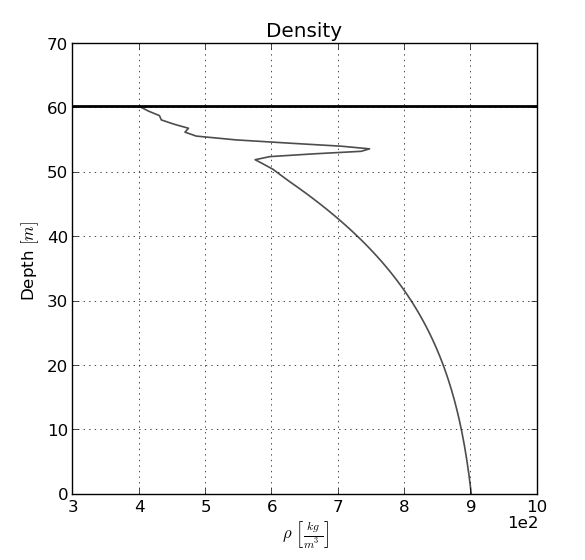
\includegraphics[width=0.42\textwidth]{images/40yrDen.png}
	\label{fig:500 year orbit}
	\caption{\footnotesize Density profile after 40 years with an ice lens approximately 7 meters below the surface}
\end{figure}

\begin{figure}[H]
	\centering
		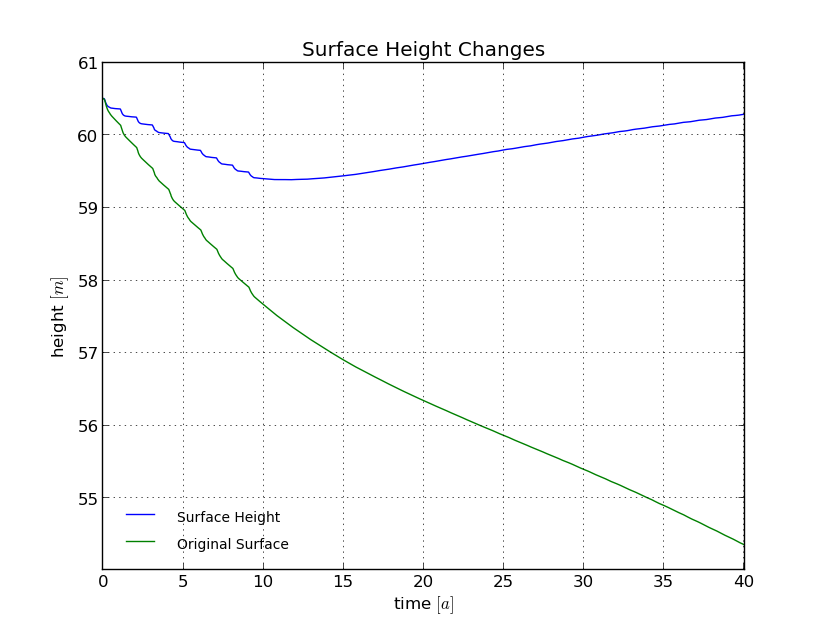
\includegraphics[width=0.42\textwidth]{images/40yrHt.png}
	\label{fig:500 year orbit}
	\caption{\footnotesize 40-year height history of the column (blue) and original surface (green) resulting in the previous figure.  This shows a rapid decrease in height as the lens is formed in the first ten years of simulation.  The fluctuations in height show an increase in height with winter temperatures.}
\end{figure}


\newpage
%% Bibliography ================================================================
\begin{thebibliography}{1}

  \bibitem{asch12}Aschwanden, A., Bueler, E., Khroulev, C., and Blatter, H. 2012. An enthalpy formulation for glaciers and ice sheets. \textit{J. Glaciol.} \textbf{58}(209), 441\mbox{-}457.
  \bibitem{pat94}Paterson, W.S.B. 1994. \textit{The physics of glaciers}, 3rd edn. Elsevier, Oxford.
  \bibitem{arth10}Arthern, R.J., Vaughan, D.G., Rankin, A.M., Mulvaney, R., and Thomas, E.R. 2010. In situ measurements of Antarctic snow compaction compared with predictions of models. \textit{J. Geophys. Res., 115}, FO3011, doi:10.1029/2009JF001306.
  \bibitem{reeh08}Reeh, N. 2008. A nonsteady\mbox{-}state firn\mbox{-}densification model for the percolation zone of a glacier. \textit{J. Geophys. Res., 113}, F03023, doi:10.1029/2007JF000746.
  \bibitem{zwa02}Zwally, H. and J. Li. 2002. Seasonal and interannual variations of firn densification and ice\mbox{-}sheet surface elevation at the Greenland summit. \textit{J. Glaciol.} \textbf{48}(161), 199\mbox{-}207.
  \bibitem{ligt11}Ligtenberg, S.R.M., Helsen, M.M., and van den Broeke, M.R. 2011. An improved semi\mbox{-}empirical model for the densification of Antarctic firn. \textit{The Cryosphere}. \textbf{5}, 809\mbox{-}819. doi:10.5194/tc\mbox{-}5\mbox{-}809\mbox{-}2011.
  \bibitem{}Coleou, C. and Lesaffre, B. 1998. Irreducible water saturation in snow: experimental results in a cold laboratory. \textit{Ann. Glaciol., 26}, 64\mbox{-}68.
  \bibitem{herr80}Herron, M. and Langway, C. 1980. Firn densification: an empirical model. \textit{J. Glaciol.} \textbf{25}(93), 373\mbox{-}385.
  \bibitem{wald02}Waldner, P.A., Schneebeli, M., Schultze \mbox{-} Zimmermann, U., and Fl\"{u}hler, H. 2002. Effect of snow structure on water flow and solute transport. \textit{Hydrol. Process.}, DOI: 10.1002/hyp.1401
  \bibitem{bozh89}Bozhinskiy, A.N. and Krass, M.S. 1989. A mathematical model of snowmelt and water percolation processes in snow and firn. \textit{Snow Cover and Glacier Variations}. IAHS publ. no. 183.
  \bibitem{logg11}Logg, A., Mardal, K., and Wells, G.N. 2011. \textit{Automated Solution of Differential Equations by the Finite Element Method}, The FEniCS Project.
\end{thebibliography}

\end{document}
%%Compile with pdflatex file.tex



